\documentclass[11pt]{article}
\usepackage{amsmath}
\usepackage{graphicx}
\usepackage{mdframed}
\usepackage[margin=0.7in]{geometry}
\usepackage[framed,numbered,autolinebreaks,useliterate]{mcode}

\begin{document}
\title{CS280 Computer Vision: HW4}
\author{Achal Dave, Richard Hwang}
\maketitle

\section{Optical Flow}
The code for generating images for a given plane, translation, and rotation is
shown in Figure \ref{optical_code}.

\begin{figure}[h!]
  \caption{Generating Images}
  \label{optical_code}
  \centering
    \begin{lstlisting}
      function draw_dynamic(X, Y, Z, t, w)
          % t, w: 3 x 1 column vectors
          % X Y Z: m x m matrices s.t. cols correspond to x values, rows to y values
          x = X ./ Z
          y = Y ./ Z
          % x y: m x m matrices
          u = zeros(size(x,2));
          v = zeros(size(y,2));
          for ix = 1:size(x,2)
              for iy = 1:size(y,2)
                  cx = x(iy, ix);
                  cy = y(iy, ix);
                  cz = Z(iy, ix);
                  trans =  (1 / cz) * [ -1 0 cx ; 0 -1 cy ] * t;
                  ang   = [cx*cy -(1 + (cx*cx)) cy ; (1 + (cy*cy)) -cx*cy -cx] * w;
                  u(iy,ix) = trans(1) + ang(1);
                  v(iy,ix) = trans(2) + ang(2);
              end
          end
          quiver(x, y, u, v)
      end
    \end{lstlisting}
\end{figure}

The code for each part is shown in Figure \ref{opt_parts_code}.
\begin{figure}[h!]
  \caption{Optical Flow Translations and Rotations}
  \label{opt_parts_code}
  \centering
    \begin{lstlisting}
      % PART A
      % speed
      ts = 5 % translation
      ws = 5 % angular

      [X, Y] = meshgrid(-5:4, ones(1,10)*-1);
      % e.g. Z(1, 5) = Z value at X = 5, Y = 1
      Z = repmat(1:10, 10, 1)';
      t = [ 0; 0; ts ];
      w = [ 0; 0; 0 ];
      figure(1)
      draw_dynamic(X, Y, Z, t, w);

      % PART B
      [X, Y] = meshgrid(-5:4, ones(1,10)*-1);
      Z = repmat(1:10, 10, 1)';
      t = [ ts ; 0 ; 0 ];
      w = [ 0 ; 0 ; 0 ];
      figure(2)
      draw_dynamic(X, Y, Z, t, w);

      % PART C
      [X, Y] = meshgrid(-5:4, ones(1,10)*-1);
      % e.g. Z(1, 5) = Z value at X = 5, Y = 1
      Z = repmat(1:10, 10, 1)';
      t = [ 0 ; ts * cos(pi / 4) ; ts * sin(pi / 4) ];
      w = [ 0 ; 0 ; 0 ];
      figure(3)
      draw_dynamic(X, Y, Z, t, w);

      % PART D
      [X, Y] = meshgrid(-5:4, -5:4);
      Z = ones(10)*2;
      t = [ 0; 0 ; 0 ];
      w = [ 1 / sqrt(2) ; 1 / sqrt(2) ; 0 ];
      figure(4)
      draw_dynamic(X, Y, Z, t, w);
    \end{lstlisting}
\end{figure}

\begin{enumerate}
\item[a)]
% this stupid thing vertically centers images
$\begin{array}{l}
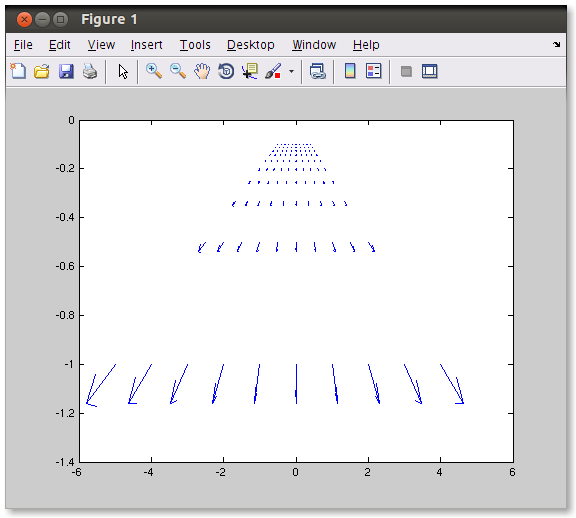
\includegraphics[width=240px]{../img/q1-a}
\end{array}$

\item[b)]
$\begin{array}{l}
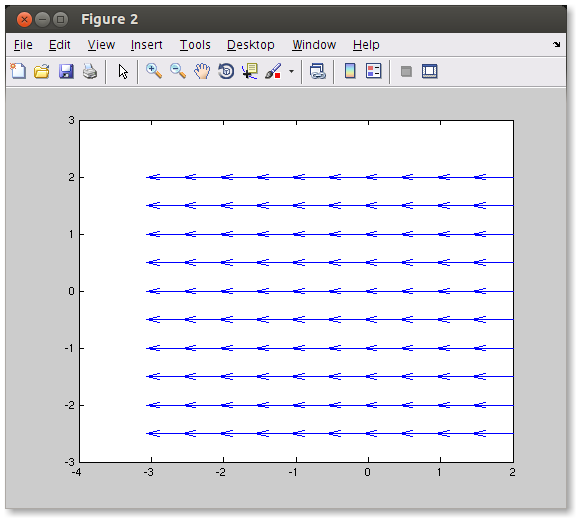
\includegraphics[width=240px]{../img/q1-b}
\end{array}$

\item[c)]
$\begin{array}{l}
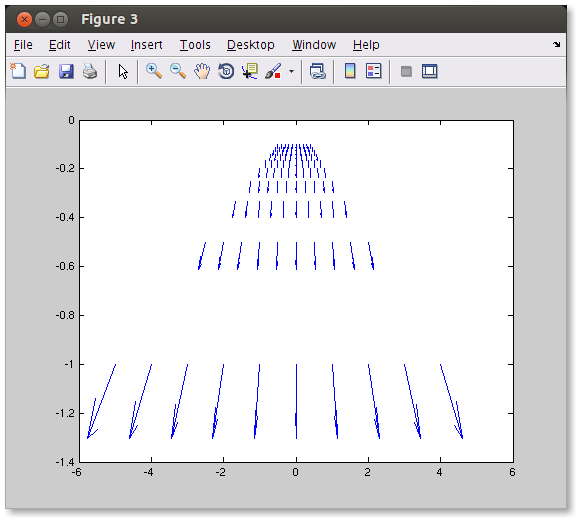
\includegraphics[width=240px]{../img/q1-c}
\end{array}$

\item[d)]
$\begin{array}{l}
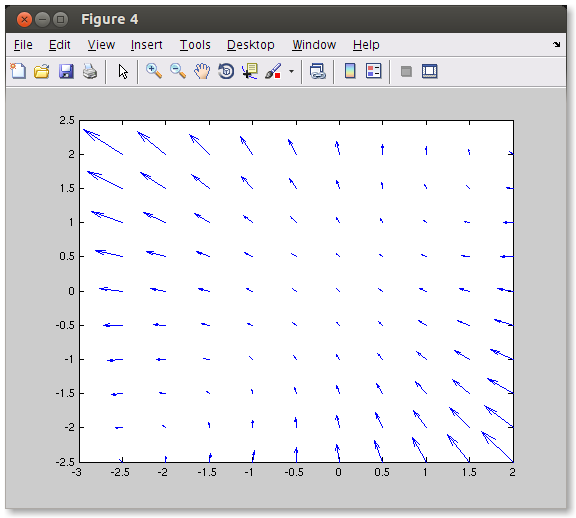
\includegraphics[width=240px]{../img/q1-d}
\end{array}$

\end{enumerate}


\newpage
\section{Error Analysis of Binocular Stereopsis}
\begin{enumerate}
\item[1.]
First, we calculate $d$ in terms of $b, f, Z$.

\begin{align*}
Z &= \frac{bf}{d} \\
d &= \frac{bf}{Z} \\
\end{align*}

Next, we can calculate $\delta Z$ in terms of $Z, \delta d$.
\begin{align*}
Z + \delta Z &= \frac{bf}{d + \delta d} \\
Z + \delta Z &= \frac{bf}{\frac{bf}{Z} + \delta d} \\
Z + \delta Z &= \frac{bfZ}{bf + (\delta d) Z} \\
\delta Z &= \frac{bfZ - bfZ - (\delta d) Z^2}{bf + (\delta d) Z} \\
\delta Z &= -\frac{(\delta d) Z^2}{bf + (\delta d) Z} \\
\end{align*}

To calculate $\delta d$, we can use the equation above to get an equation for
$\delta d$. Rearranging the terms, we get

\begin{align*}
\delta d = \frac{\delta Z * bf}{Z^2 + Z \delta Z}
\end{align*}

From here, the code is relatively simple:
\begin{verbatim}
deltad = (err * b * f) ./ (z .* (z + err));
\end{verbatim}

\end{enumerate}


\newpage
\section{Multi-View Reconstruction}
\subsection{Finding the Fundamental Matrix}
We followed the eight point algorithm. First, we normalize all the points by
translating them by $\mu$ and scaling them such that the mean distance from
$\mu$ (the new origin) is $\sqrt{2}$. Next, we compute $A$, a $N\times$ matrix.
We want $Af = 0$ as this is just $x_2^tFx_1 = 0$ rewritten, but there is noise.
We solve $min_f||Af||_2$, then, by taking the right singular vector of $A$
corresponding to the smallest singular value. This is our $F_{est}$. We must
enforce that the fundamental matrix is of rank 2. So, we solve
$min_F||F-F_{est}||_F$, via SVD. If $F_{est} = USV_t$, then $F = U\hat{S}V^t$,
where $\hat{S} = diag(s_1, s_2, 0)$. The fundamental matrices we found with
this method are shown in Figures \ref{f_lib} and \ref{f_house}.

Thus, to answer the question posed, we are minimizing the residual error.
This is because F is defined as $e_2 = Fx_1$, where $e_2$ is the epipolar line
for camera two.  $x_2^tFx_1$ should be zero, then, if $x_2$ lies on $e_2$. The
optimization problem is trying to get $x_2$ as close as possible to on $e_2$.

Our definition of the residual is the mean squared distance between the points
in the two images and the corresponding lines. Calculation of the residual
error is shown in Figure \ref{residual_code}. For the library image,
we found a residual error of 0.096304, while for the house image, we found
a residual error of 0.806142.

\begin{figure}[h!]
  \caption{Fundamental Matrix for Library}
  \label{f_lib}
  \centering
    $\begin{pmatrix}
      -0.0000&0.0004&-0.0200\\
      -0.0005&0.0000&0.4109\\
      0.0697&-38.96&-9.2135
    \end{pmatrix}$
\end{figure}
\begin{figure}[h!]
  \caption{Fundamental Matrix for House}
  \label{f_house}
  \centering
    $\begin{pmatrix}
      0.0000&0.0002&-0.0523\\
      0.0003&0.0000&-0.7753\\
      0.0280&0.6763& 4.6626
    \end{pmatrix}$
\end{figure}

\begin{figure}[h!]
  \caption{Calculation of Residual Error}
  \label{residual_code}
  \centering
    \begin{lstlisting}
      % Compute mean squared distance between points in their two images and their
      % corresponding epipolar lines.
      dist_sum = 0;
      for i = 1:N
          x_1 = [matches(i, 1:2) 1]';
          x_2 = [matches(i, 3:4) 1]';
          el_1 = F' * x_2;
          el_2 = F * x_1;
          
          a_1 = el_1(1);
          b_1 = el_1(2);
          c_1 = el_1(3);
          dist_1 = abs(a_1*x_1(1) + b_1*x_1(2) + c_1) / sqrt(a_1^2 + b_1^2);

          a_2 = el_2(1);
          b_2 = el_2(2);
          c_2 = el_2(3);
          dist_2 = abs(a_2*x_2(1) + b_2*x_2(2) + c_2) / sqrt(a_2^2 + b_2^2);

          % calc distance of x_1 from el_1, and x_2 from el_2
          dist_sum = dist_sum + dist_1^2 + dist_2^2;
      end

      res_err = dist_sum / (2*N);
    \end{lstlisting}
\end{figure}

\newpage
\subsection{Finding the Camera Rotation and Translation}
All possible possibilities for $t$ and $R$ for the two images are shown in
Figures \ref{tr_library} and \ref{tr_house}.

\begin{figure}[h!]
  \caption{ts and Rs for Library}
  \label{tr_library}
  \centering
    \[t = \begin{pmatrix}
      -0.7882\\
      0.1562\\
      0.5953
    \end{pmatrix}, 
    \begin{pmatrix}
      0.7882\\
      -0.1562\\
      -0.5953
    \end{pmatrix}\]

    \[R = \begin{pmatrix}
      -0.9941&-0.0568&0.0924\\
       0.0525&-0.9975&-0.0482\\
      -0.0949& 0.0430&-0.9946
    \end{pmatrix},
    \begin{pmatrix}
      -0.1649&0.1915&0.9675\\
      0.1772& 0.9708&-0.1619\\
      0.9703&-0.1447&0.1940
    \end{pmatrix}\]
\end{figure}

\begin{figure}[h!]
  \caption{ts and Rs for House}
  \label{tr_house}
  \centering
    \[t = \begin{pmatrix}
      0.9975\\
      0.0326\\
      0.0621
    \end{pmatrix}, 
    \begin{pmatrix}
      -0.9975\\
      -0.0326\\
      -0.0621
    \end{pmatrix}\]

    \[R = \begin{pmatrix}
      0.9822&0.0627&-0.1771\\
     -0.0641&0.9979&-0.0017\\
      0.1766&0.0130&0.9842
    \end{pmatrix},
    \begin{pmatrix}
      0.9903&0.1286&-0.0534\\
      0.1285&-0.9917&-0.0058\\
      -0.0537&-0.0011&-0.9986
    \end{pmatrix}\]
\end{figure}


\subsection{Reconstruction of 3D Point Cloud}
We are directly trying to minimize the reconstruction error. We rewrite

\begin{align*}
  x &= PX\\
  y &= PY
\end{align*}

into $Ax = 0$ and try to find $x = \begin{pmatrix}X\\Y\\Z\\W\end{pmatrix}$
that minimizes $Ax$. Calculation of the reconstruction error for one pair of
points is shown in Figure \ref{reconstruction_code}. Reconstruction errors for
the library and house are 4.204884 and 2.323244.

\begin{figure}[h!]
  \caption{Calculation of Reconstruction Error}
  \label{reconstruction_code}
  \centering
    \begin{lstlisting}
      proj_1 = P1 * point;
      proj_1 = proj_1(1:2, :) ./ proj_1(3,1);

      proj_2 = P2 * point;
      proj_2 = proj_2(1:2, :) ./ proj_2(3,1);

      % Compute distances.
      errs(1+i*2) = sqrt(sum((x_1.' - proj_1).^2));
      errs(2+i*2) = sqrt(sum((x_2.' - proj_2).^2));
    \end{lstlisting}
\end{figure}


\subsection{Plotting the 3D Point Cloud}
The scatter plots for each image are shown in Figures \ref{3d_lib} and
\ref{3d_house}. In Figure \ref{3d_lib}, we note that the points lie mostly
in one plane, which corresponds to the library wall. We also notice the spots
around the bushes at the base of the library wall. In Figure \ref{3d_house},
we present a bird's eye view. To the left, we note the points on the rug.
Especially noticable are corner and walls of the house.

\begin{figure}[h!]
  \caption{3D Point Cloud for Library}
  \label{3d_lib}
  \centering
    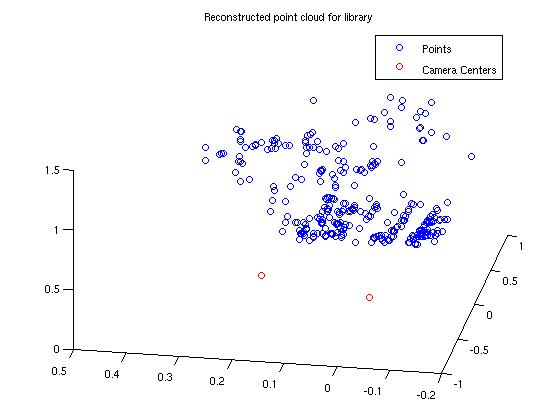
\includegraphics[width=0.6\linewidth]{../img/library_camera.jpg}
\end{figure}

\begin{figure}[h!]
  \caption{3D Point Cloud for House}
  \label{3d_house}
  \centering
    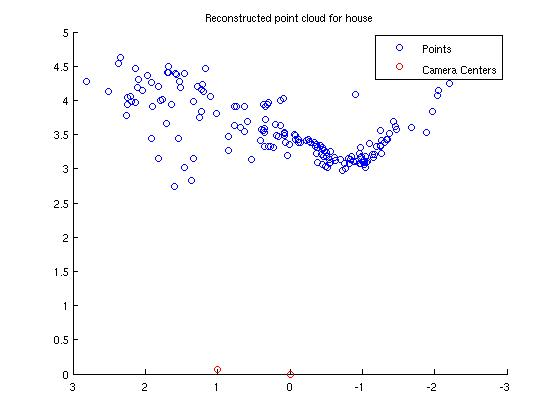
\includegraphics[width=0.6\linewidth]{../img/house_camera.jpg}
\end{figure}

\end{document}
